\begin{examplebox}
\textbf{\textcolor{CExample}{例 1（先体验它解决了什么：直线上的动点、动直线与定点）}}

\textbf{题目：} 已知圆 $x^2+y^2=4$ 和固定点 $P(4,0)$。点 $Q$ 在直线 $x=1$ 上运动。
（1）写出 $P$ 的极线；（2）设 $Q(1,t)$，写出 $Q$ 的极线；（3）证明这些动直线都经过同一固定点；（4）分别讨论 $t=0,\sqrt3,2$ 的几何意义。

\textbf{详细解答：}
\begin{description}[style=nextline,leftmargin=2.8em,itemsep=0.45em]
\item[\textbf{第一步：判断固定直线从哪来。}] 对圆 $x^2+y^2=4$，点 $P(4,0)$ 的极线满足 $4x+0y=4$，即 $l_P:x=1$。所以题目中的固定直线\textbf{刚好就是 $P$ 的极线}。
\item[\textbf{第二步：给动点配直线。}] 因为 $Q$ 在 $x=1$ 上，可设 $Q(1,t)$。圆的极线公式是 $x_Qx+y_Qy=4$，代入 $x_Q=1,y_Q=t$，得到
\[\boxed{l_Q:x+ty=4}.\]
\item[\textbf{第三步：证明过定点。}] 把 $P(4,0)$ 代入：$4+t\cdot0=4$。无论 $t$ 怎么变化都成立，所以 $l_Q$ 始终经过 $P(4,0)$。
\item[\textbf{第四步：解释 $Q$ 的三个位置。}]
$Q(1,0)$ 满足 $1^2+0^2<4$，所以在圆内，其极线 $x=4$ 与圆不相交；
$Q(1,\sqrt3)$ 满足 $1+3=4$，在圆上，其极线 $x+\sqrt3y=4$ 是圆在 $Q$ 处的切线；
$Q(1,2)$ 满足 $1+4>4$，在圆外，其极线 $x+2y=4$ 是该外点的两条切线的两个切点的连线。
\end{description}
\textbf{本例最重要的收获：} $Q$ 在圆内、圆上、圆外都不影响“$l_Q$ 经过 $P$”的证明；\textbf{改变的是极线与圆的交点情况，不是点线互换的代数关系。}

\medskip
\textbf{\textcolor{CExample}{例 2（真正有价值的切点弦过定点题）}}

\textbf{题目：} 已知圆 $x^2+y^2=4$。动点 $Q(1,t)$ 在圆外，即 $|t|>\sqrt3$。从 $Q$ 向圆作两条切线，切点为 $T_1,T_2$。证明：\textbf{直线 $T_1T_2$ 恒经过定点 $(4,0)$}。


\begin{center}
\begin{tikzpicture}[x=1.15cm,y=1.15cm,every node/.style={font=\small}]
\draw[blue!75!black,thick] (0,0) circle (2);
\draw[red!75!black,dashed,thick] (1,-2.3)--(1,2.8);
\draw[orange!80!black,very thick] (-.6,2.3)--(4.5,-.25);
\draw[gray!75,thick] (1,2)--(0,2) (1,2)--(1.6,1.2);
\fill (0,2) circle (2pt) node[above left=4pt] {$T_1(0,2)$};
\fill (1.6,1.2) circle (2pt);\node at (-.5,.6) {$T_2(\frac85,\frac65)$};
\fill (1,2) circle (2pt) node[above right=5pt] {$Q(1,2)$};
\fill (4,0) circle (2pt) node[below=5pt] {$P(4,0)$};
\node[orange!80!black] at (3.4,1.5) {$T_1T_2:x+2y=4$};
\node at (1,-2.9) {定点 $P$ 在切点弦的延长线上，不必在线段 $T_1T_2$ 上。};
\end{tikzpicture}

\end{center}
图取 $t=2$：灰色为两条切线段，橙色为切点弦所在直线。

\textbf{解法甲：先识别结构，速度最快。}
\begin{description}[style=nextline,leftmargin=2.8em,itemsep=0.4em]
\item[\textbf{第一步：认出切点弦。}] 对圆外点 $Q(1,t)$，两切点的连线就是 $Q$ 的极线，即 $T_1T_2:x+ty=4$。
\item[\textbf{第二步：找出定点。}] 把 $(4,0)$ 代入，得到 $4+t\cdot0=4$，所以直线 $T_1T_2$ 恒经过 $(4,0)$。
\item[\textbf{第三步：解释为什么会想到 $(4,0)$。}] 因为 $Q$ 在固定直线 $x=1$ 上，而 $x=1$ 正是点 $P(4,0)$ 的极线；所以先想到 $T_1T_2$ 会经过 $P$，随后代入验证即可。
\end{description}
\textbf{解法乙：不使用“极线”这个名称，也能得到同一结论。}

设任一切点为 $T(x,y)$。切线处的半径 $OT\perp QT$，故
\[
OQ^2=OT^2+QT^2.
\]
由于 $Q(1,t)$，$OQ^2=1+t^2$；而 $OT^2=4$，$QT^2=(x-1)^2+(y-t)^2$，所以
\[
1+t^2=4+(x-1)^2+(y-t)^2.
\]
展开右边：
\[
4+x^2-2x+1+y^2-2ty+t^2.
\]
整理后得到 $0=4+x^2+y^2-2x-2ty$。切点在圆上，$x^2+y^2=4$，因此
\[0=8-2x-2ty,\qquad\boxed{x+ty=4}.\]
两个切点都满足这个一次方程，所以切点弦就是 $x+ty=4$，再次代入 $(4,0)$ 得证。

\textbf{方法比较：} 直接作勾股计算完全符合高中知识要求；懂得极线后，可以提前认出这一套计算每次\textbf{都会得到什么形式}。这就是学习本结论的实际收益。

\medskip
\textbf{\textcolor{CExample}{例 3（保留原题：椭圆上两个点互在极线上）}}

\textbf{题目：} 椭圆 $\frac{x^2}{4}+y^2=1$，点 $P(2,0)$ 与 $Q(2,1)$。（1）求两点的极线；（2）验证它们互在对方的极线上。

\textbf{解：} 对椭圆，$R(u,v)$ 的极线是 $\frac{ux}{4}+vy=1$，故
\[
l_P:\frac{2x}{4}=1\iff x=2;
\qquad l_Q:\frac{2x}{4}+y=1\iff\frac{x}{2}+y=1.
\]
代入 $Q(2,1)$ 到 $l_P$：$x=2$ 成立。代入 $P(2,0)$ 到 $l_Q$：$2/2+0=1$，也成立。或直接观察
\[
\frac{2\cdot2}{4}+0\cdot1=1.
\]
\textbf{几何意义：} $P(2,0)$ 本来就在椭圆上，所以 $l_P:x=2$ 是椭圆在最右端点的切线。$Q(2,1)$ 在这条切线上却不在椭圆上；由互换关系，$Q$ 的极线必经过切点 $P$。

\medskip
\textbf{\textcolor{CExample}{例 4（椭圆：圆内对应的思想怎么迁移？）}}

\textbf{题目：} 椭圆 $\frac{x^2}{9}+\frac{y^2}{4}=1$，固定点 $P(2,0)$ 在椭圆内部。动点 $Q$ 沿直线 $x=\frac92$ 移动。
（1）证明这条固定直线是 $P$ 的极线；（2）证明每个 $Q$ 对应的极线都经过 $P$；（3）说明 $Q$ 在椭圆外时，这个结论有什么更直观的说法。


\begin{center}
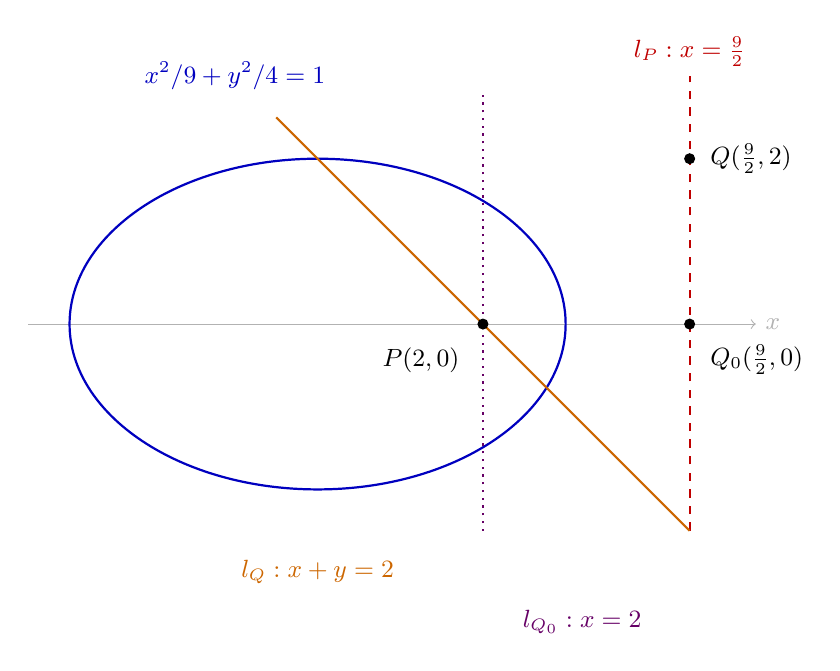
\begin{tikzpicture}[x=1.05cm,y=1.05cm,every node/.style={font=\small}]
\draw[->,gray!60] (-3.5,0)--(5.3,0) node[right] {$x$};
\draw[blue!75!black,thick] (0,0) ellipse (3 and 2);
\draw[red!75!black,dashed,thick] (4.5,-2.5)--(4.5,3);
\draw[orange!80!black,thick] (-.5,2.5)--(4.5,-2.5);
\draw[violet!80!black,dotted,thick] (2,-2.5)--(2,2.8);
\fill (2,0) circle (2pt) node[below left=5pt] {$P(2,0)$};
\fill (4.5,2) circle (2pt) node[right=4pt] {$Q(\frac92,2)$};
\fill (4.5,0) circle (2pt) node[below right=4pt] {$Q_0(\frac92,0)$};
\node[red!75!black,above] at (4.5,3) {$l_P:x=\frac92$};
\node[orange!80!black] at (0,-3) {$l_Q:x+y=2$};
\node[violet!80!black] at (3.2,-3.6) {$l_{Q_0}:x=2$};
\node[blue!75!black] at (-1,3) {$x^2/9+y^2/4=1$};
\end{tikzpicture}

\end{center}
图取 $t=0,2$：$P$ 在椭圆内部，动点所在的固定直线在椭圆外部。

\textbf{解：}
\begin{description}[style=nextline,leftmargin=2.8em,itemsep=0.42em]
\item[\textbf{第一步：判断 $P$ 的位置。}] 将 $P(2,0)$ 代入椭圆左边：$4/9+0<1$，所以 $P$ 在椭圆内部。\textbf{这时不能}说从 $P$ 向椭圆作两条真实切线。
\item[\textbf{第二步：写出 $P$ 的极线。}] $l_P:\frac{2x}{9}+0y=1$，化简得 $x=\frac92$。因此题目给定的动点直线正好是 $l_P$。
\item[\textbf{第三步：设动点并写极线。}] 取 $Q(\frac92,t)$，那么
\[
l_Q:\frac{\frac92 x}{9}+\frac{ty}{4}=1,
\quad\text{即}\quad\boxed{\frac{x}{2}+\frac{ty}{4}=1}.
\]
\item[\textbf{第四步：验定点。}] 把 $P(2,0)$ 代入，左侧为 $\frac22+\frac{t\cdot0}{4}=1$，恒成立。所以每条 $l_Q$ 都经过 $P(2,0)$。
\item[\textbf{第五步：翻译成常见图形语言。}] 因为 $x_Q=\frac92>3$，每个 $Q$ 都在椭圆外，可以从 $Q$ 向椭圆作两条切线。两个切点的连线正是 $l_Q$，所以\textbf{这些切点弦都经过椭圆内部的同一个定点 $(2,0)$}。
\end{description}
\textbf{顿悟：} 一个点虽然在椭圆内部、不能画出它的两条切线，但它仍能通过“自己的极线”控制\textbf{一整组椭圆外点的切点弦}。这就是统一公式的几何力量。

\medskip
\textbf{\textcolor{CExample}{例 5（保留原题：抛物线不需要排除中心点）}}

\textbf{题目：} 抛物线 $y^2=2x$，$P(2,2)$，$Q(-2,0)$。（1）验证 $P,Q$ 互在对方的极线上；（2）若 $R$ 在直线 $x=-1$ 上，且 $R$ 在 $P$ 的极线上，求 $R$。

\textbf{解：} 对抛物线 $y^2=2x$，点 $W(u,v)$ 的极线为
\[\boxed{vy=x+u}.\]
所以 $P$ 的极线为 $l_P:2y=x+2$。代入 $Q(-2,0)$：$2\cdot0=(-2)+2=0$，成立。另一方面，$Q$ 的极线为 $0\cdot y=x-2$，即 $x=2$，代入 $P(2,2)$ 也成立。

设 $R(-1,t)$，因为 $R\in l_P$，所以
\[2t=(-1)+2=1,\qquad t=\frac12.\]
因此 $R\left(-1,\frac12\right)$。反向核验：$R$ 的极线为 $\frac12y=x-1$，代入 $P(2,2)$：$\frac12\cdot2=2-1$，成立。

\textbf{识别要点：} 抛物线用的是 $y_1y_2=x_1+x_2$，\textbf{不是} $x_1x_2+y_1y_2=r^2$。曲线不同，具体公式不同；相同的是交换两点后等式不变。

\medskip
\textbf{\textcolor{CExample}{例 6（双曲线：减号会不会破坏互换关系？）}}

\textbf{题目：} 双曲线 $\frac{x^2}{4}-\frac{y^2}{9}=1$，点 $P(4,0)$，点 $Q(1,3)$。求 $l_P,l_Q$，判断是否互在对方的极线上。

\textbf{解：} 对点 $W(u,v)$，极线为 $\frac{ux}{4}-\frac{vy}{9}=1$。故
\[
l_P:\frac{4x}{4}=1\iff x=1,
\qquad
l_Q:\frac{x}{4}-\frac{3y}{9}=1\iff\frac{x}{4}-\frac{y}{3}=1.
\]
将 $Q(1,3)$ 代入 $l_P$，$x=1$ 成立；将 $P(4,0)$ 代入 $l_Q$，$4/4-0=1$，也成立。

\textbf{为什么不受减号影响？} 两点之间的判断式是 $\frac{x_1x_2}{4}-\frac{y_1y_2}{9}=1$；交换两点时，\textbf{每一项内部只交换乘法次序}，原来的减号没有变化。

\medskip
\textbf{\textcolor{CExample}{例 7（保留原题：已知直线反求对应的点）}}

\textbf{题目：} 椭圆 $\frac{x^2}{9}+\frac{y^2}{4}=1$，直线 $l:x=3$。（1）求极线恰好为 $l$ 的点 $P$；（2）给定 $Q(3,2)$，说明它与 $P$ 的对应关系。

\textbf{解：} 设 $P(u,v)$，则 $l_P:\frac{ux}{9}+\frac{vy}{4}=1$。因为此直线要与 $x=3$ 是同一条直线，即 $\frac{x}{3}=1$，可比较得到 $\frac{u}{9}=\frac13$，$\frac{v}{4}=0$，所以 $u=3,v=0$，得 $P(3,0)$。

$Q(3,2)$ 满足 $x=3$，所以 $Q\in l_P$。由互换关系，$P\in l_Q$。如要直接检验，$l_Q:\frac{3x}{9}+\frac{2y}{4}=1$，即 $\frac{x}{3}+\frac{y}{2}=1$，代入 $(3,0)$ 成立。

\textbf{必须区分：} “求极点”是\textbf{由直线反推对应的点}；“证明共轭”是\textbf{证明两点各自在对方对应的直线上}。它们有关联，但不是同一个问题。

\medskip
\textbf{\textcolor{CExample}{例 8（高价值变式：不给定点，能不能找出来？）}}

\textbf{题目：} 对圆 $x^2+y^2=4$，动点 $Q$ 位于 $2x+y=4$ 上。已知这条直线确实是某个点的极线。求这个固定点 $P$，并证明 $Q$ 的极线均经过 $P$。

\textbf{解：} 设 $P(u,v)$，则 $l_P:ux+vy=4$。比较 $2x+y=4$，可直接得到 $u=2,v=1$，所以 $P(2,1)$。\textbf{注意} $P$ 在圆外，因为 $2^2+1^2=5>4$。

设动点 $Q(s,t)$，由 $Q\in 2x+y=4$ 得 $2s+t=4$；其极线为 $l_Q:sx+ty=4$。将 $P(2,1)$ 代入 $l_Q$，左侧是 $2s+t=4$，恰好由题目条件保证，所以 $P$ 是定点。

\textbf{迁移提醒：} 当定直线为 $2x+y=4$ 时，固定点并非直线上的点，而是由\textbf{“这条直线是谁的极线”}反推出来。对于圆 $x^2+y^2=4$，$ux+vy=4$ 的系数直接给出对应点 $(u,v)$；换成椭圆或双曲线，必须按对应分母恢复坐标。
\end{examplebox}
